
\documentclass[12pt]{article}
\usepackage{amsmath,amssymb}
\usepackage{tcolorbox}
\usepackage{tikz}
\usepackage{geometry}
\geometry{margin=1in}
\title{Chapter 6: Complete Study Guide \\ Examples 6-1 to 6-24 and Problems P.6-1 to P.6-53}
\author{}
\date{}
\begin{document}
\maketitle
\tableofcontents
\newpage

\section*{Chapter 6 Summary: Static Magnetic Fields}

\subsection*{Key Concepts}
\begin{itemize}
  \item Magnetic fields are generated by steady currents.
  \item The primary tools to analyze static magnetic fields are Biot–Savart Law and Ampère’s Law.
  \item Magnetic flux density: \( \vec{B} \), Magnetic field intensity: \( \vec{H} \)
  \item Related via \( \vec{B} = \mu \vec{H} \), where \( \mu \) is the permeability of the medium.
  \item Vector potential \( \vec{A} \) is defined such that \( \vec{B} = \nabla \times \vec{A} \)
\end{itemize}

\subsection*{Important Laws and Equations}
\begin{itemize}
  \item \textbf{Biot–Savart Law:}
  \[
  \vec{B} = \frac{\mu_0}{4\pi} \int \frac{I\, d\vec{l} \times \hat{r}}{r^2}
  \]
  
  \item \textbf{Ampère’s Law:}
  \[
  \oint \vec{H} \cdot d\vec{l} = I_{\text{enc}}
  \]

  \item \textbf{Boundary Conditions:}
  \[
  \hat{n} \cdot (\vec{B}_2 - \vec{B}_1) = 0, \quad
  \hat{n} \times (\vec{H}_2 - \vec{H}_1) = \vec{K}_s
  \]

  \item \textbf{Magnetic Vector Potential:}
  \[
  \vec{B} = \nabla \times \vec{A}
  \]

  \item \textbf{Inductance and Energy:}
  \[
  \Phi = L I, \quad W = \frac{1}{2} L I^2, \quad u = \frac{1}{2} \vec{B} \cdot \vec{H}
  \]
\end{itemize}

\subsection*{Magnetic Materials}
\begin{itemize}
  \item \( \vec{B} = \mu_0 (\vec{H} + \vec{M}) \)
  \item Bound currents: \( \vec{J}_b = \nabla \times \vec{M}, \quad \vec{K}_b = \vec{M} \times \hat{n} \)
  \item Magnetic dipoles and forces: \( \vec{\tau} = \vec{m} \times \vec{B} \)
\end{itemize}

\subsection*{Magnetic Circuits}
\begin{itemize}
  \item Magnetic reluctance: \( \mathcal{R} = \frac{l}{\mu A} \)
  \item Magnetic analogs to electrical circuits: \( \Phi = \frac{\text{mmf}}{\mathcal{R}} \)
\end{itemize}

\newpage


\section*{Examples 6-1 to 6-4: Fully Worked Solutions}

\subsection*{Example 6-1: Field at the Center of a Circular Loop}

\textbf{Problem:}  
Find \( \vec{H} \) at the center of a circular loop of radius \( R \) carrying current \( I \).

\textbf{Solution:}

Using Biot–Savart Law:

\[
\vec{B} = \frac{\mu_0 I}{4\pi} \int \frac{d\vec{l} \times \hat{r}}{r^2}
\]

At the center, all elements contribute equally in the \( \hat{z} \)-direction:

\[
\vec{B} = \frac{\mu_0 I}{2R} \hat{z}
\Rightarrow \vec{H} = \frac{\vec{B}}{\mu_0} = \frac{I}{2R} \hat{z}
\]

\begin{tcolorbox}
\[
\boxed{\vec{B} = \frac{\mu_0 I}{2R} \hat{z}}, \quad
\boxed{\vec{H} = \frac{I}{2R} \hat{z}}
\]
\end{tcolorbox}

\subsection*{Example 6-2: Field on Axis of a Loop}

\textbf{Problem:}  
Find \( B_z \) at point \( z \) on the axis of a current loop of radius \( R \).

\textbf{Solution:}

Using Biot–Savart Law:

\[
B_z = \frac{\mu_0 I R^2}{2 (R^2 + z^2)^{3/2}}
\]

\begin{tcolorbox}
\[
\boxed{B_z = \frac{\mu_0 I R^2}{2 (R^2 + z^2)^{3/2}}}
\]
\end{tcolorbox}

\subsection*{Example 6-3: Field Inside a Long Straight Wire}

\textbf{Problem:}  
Find \( \vec{H} \) inside a conductor of radius \( a \), uniformly carrying current \( I \).

\textbf{Solution:}

\[
J = \frac{I}{\pi a^2}, \quad I_{\text{enc}} = J \pi r^2 = I \frac{r^2}{a^2}
\]

Using Ampère’s Law:
\[
H \cdot 2\pi r = I_{\text{enc}} \Rightarrow H = \frac{I r}{2\pi a^2}
\]

\begin{tcolorbox}
\[
\boxed{\vec{H} = \frac{I r}{2\pi a^2} \hat{\phi}}, \quad r < a
\]
\end{tcolorbox}

\subsection*{Example 6-4: Field Outside the Same Wire}

\textbf{Problem:}  
Find \( \vec{H} \) outside the wire \( (r > a) \).

\textbf{Solution:}

Total current enclosed is \( I \):

\[
H \cdot 2\pi r = I \Rightarrow H = \frac{I}{2\pi r}
\]

\begin{tcolorbox}
\[
\boxed{\vec{H} = \frac{I}{2\pi r} \hat{\phi}}, \quad r > a
\]
\end{tcolorbox}



\section*{Examples 6-5 to 6-8: Fully Worked Solutions}

\subsection*{Example 6-5: Magnetic Field in Cylindrical Region with Uniform J}

\textbf{Problem:}  
A long cylinder of radius \( a \) carries a uniform current density \( \vec{J} = J \hat{z} \). Find \( \vec{B}(r) \) inside the cylinder.

\textbf{Solution:}

Using Ampère’s Law:
\[
\oint \vec{B} \cdot d\vec{l} = \mu_0 I_{\text{enc}}
\]

\[
I_{\text{enc}} = J \pi r^2 \quad \Rightarrow \quad B \cdot 2\pi r = \mu_0 J \pi r^2
\Rightarrow B = \frac{\mu_0 J r}{2}
\]

\begin{tcolorbox}
\[
\boxed{\vec{B}(r) = \frac{\mu_0 J r}{2} \hat{\phi}}, \quad r < a
\]
\end{tcolorbox}

\subsection*{Example 6-6: Magnetic Field Outside the Same Cylinder}

\textbf{Problem:}  
Find \( \vec{B}(r) \) for \( r > a \).

\textbf{Solution:}

\[
I_{\text{enc}} = J \pi a^2, \quad B \cdot 2\pi r = \mu_0 J \pi a^2
\Rightarrow B = \frac{\mu_0 J a^2}{2r}
\]

\begin{tcolorbox}
\[
\boxed{\vec{B}(r) = \frac{\mu_0 J a^2}{2r} \hat{\phi}}, \quad r > a
\]
\end{tcolorbox}

\subsection*{Example 6-7: Coaxial Cable Field Distribution}

\textbf{Problem:}  
A coaxial cable has inner radius \( a \), outer radius \( b \), with current \( I \) flowing through inner and returning through outer. Find \( \vec{B}(r) \) for each region.

\textbf{Solution:}

- \( r < a \): \( B = \frac{\mu_0 I r}{2\pi a^2} \)
- \( a < r < b \): \( B = \frac{\mu_0 I}{2\pi r} \)
- \( r > b \): net enclosed current is zero → \( B = 0 \)

\begin{tcolorbox}
\[
\boxed{
\vec{B}(r) =
\begin{cases}
\frac{\mu_0 I r}{2\pi a^2} \hat{\phi}, & r < a \\
\frac{\mu_0 I}{2\pi r} \hat{\phi}, & a < r < b \\
0, & r > b
\end{cases}
}
\]
\end{tcolorbox}

\subsection*{Example 6-8: B-Field from Surface Current on a Sheet}

\textbf{Problem:}  
A sheet in the \( yz \)-plane carries surface current density \( \vec{K} = K \hat{y} \). Find \( \vec{B} \) on both sides.

\textbf{Solution:}

Ampère’s Law around rectangular path crossing the sheet:
\[
\vec{B}_{\text{above}} - \vec{B}_{\text{below}} = \mu_0 \vec{K} \times \hat{n}
\Rightarrow \vec{B} = \pm \frac{\mu_0 K}{2} \hat{z}
\]

\begin{tcolorbox}
\[
\boxed{
\vec{B} =
\begin{cases}
\frac{\mu_0 K}{2} \hat{z}, & x > 0 \\
-\frac{\mu_0 K}{2} \hat{z}, & x < 0
\end{cases}
}
\]
\end{tcolorbox}



\section*{Examples 6-9 to 6-12: Fully Worked Solutions}

\subsection*{Example 6-9: Magnetic Vector Potential from Infinite Wire}

\textbf{Problem:}  
Find the magnetic vector potential \( \vec{A} \) for an infinite straight wire carrying current \( I \).

\textbf{Solution:}

In cylindrical coordinates:
\[
\vec{A} = \frac{\mu_0 I}{2\pi} \ln r \, \hat{z}
\]
Since:
\[
\vec{B} = \nabla \times \vec{A} = \frac{\mu_0 I}{2\pi r} \hat{\phi}
\]

\begin{tcolorbox}
\[
\boxed{\vec{A} = \frac{\mu_0 I}{2\pi} \ln r \, \hat{z}}
\]
\end{tcolorbox}

\subsection*{Example 6-10: Field from a Magnetic Dipole}

\textbf{Problem:}  
Find \( \vec{B} \) due to a magnetic dipole \( \vec{m} \) at the origin.

\textbf{Solution:}

The magnetic field is:
\[
\vec{B} = \frac{\mu_0}{4\pi} \left( \frac{3(\vec{m} \cdot \hat{r})\hat{r} - \vec{m}}{r^3} \right)
\]

\begin{tcolorbox}
\[
\boxed{
\vec{B} = \frac{\mu_0}{4\pi} \left( \frac{3(\vec{m} \cdot \hat{r})\hat{r} - \vec{m}}{r^3} \right)
}
\]
\end{tcolorbox}

\subsection*{Example 6-11: Inductance of a Solenoid}

\textbf{Problem:}  
Find the inductance \( L \) of a solenoid with \( N \) turns, length \( l \), and cross-sectional area \( A \).

\textbf{Solution:}

\[
B = \mu_0 \frac{N}{l} I, \quad \Phi = B A = \mu_0 \frac{N}{l} I A
\Rightarrow L = \frac{N \Phi}{I} = \frac{\mu_0 N^2 A}{l}
\]

\begin{tcolorbox}
\[
\boxed{L = \frac{\mu_0 N^2 A}{l}}
\]
\end{tcolorbox}

\subsection*{Example 6-12: Energy Stored in Magnetic Field of Solenoid}

\textbf{Problem:}  
Find magnetic energy stored in the solenoid above.

\textbf{Solution:}

\[
W = \frac{1}{2} L I^2 = \frac{1}{2} \cdot \frac{\mu_0 N^2 A}{l} \cdot I^2
= \frac{\mu_0 N^2 A I^2}{2l}
\]

\begin{tcolorbox}
\[
\boxed{W = \frac{\mu_0 N^2 A I^2}{2l}}
\]
\end{tcolorbox}



\section*{Examples 6-13 to 6-16: Fully Worked Solutions}

\subsection*{Example 6-13: Energy Density in Magnetic Field}

\textbf{Problem:}  
Express the energy density of a magnetic field in a material of permeability \( \mu \).

\textbf{Solution:}

Magnetic energy density:
\[
u = \frac{1}{2} \vec{B} \cdot \vec{H} = \frac{1}{2} \mu H^2
\]

\begin{tcolorbox}
\[
\boxed{u = \frac{1}{2} \mu H^2}
\]
\end{tcolorbox}

\subsection*{Example 6-14: Magnetic Force on Wire in Field}

\textbf{Problem:}  
Find the force on a wire of length \( L \), current \( I \), in magnetic field \( \vec{B} \).

\textbf{Solution:}

\[
\vec{F} = I \vec{L} \times \vec{B}
\]

\begin{tcolorbox}
\[
\boxed{\vec{F} = I \vec{L} \times \vec{B}}
\]
\end{tcolorbox}

\subsection*{Example 6-15: Torque on a Magnetic Dipole}

\textbf{Problem:}  
A magnetic dipole \( \vec{m} \) is placed in magnetic field \( \vec{B} \). Find torque.

\textbf{Solution:}

\[
\vec{\tau} = \vec{m} \times \vec{B}
\]

\begin{tcolorbox}
\[
\boxed{\vec{\tau} = \vec{m} \times \vec{B}}
\]
\end{tcolorbox}

\subsection*{Example 6-16: Magnetic Scalar Potential}

\textbf{Problem:}  
When can a magnetic scalar potential \( \psi_m \) be defined?

\textbf{Solution:}

If \( \vec{J} = 0 \), then \( \nabla \times \vec{H} = 0 \), so:

\[
\vec{H} = -\nabla \psi_m
\]

\begin{tcolorbox}
\[
\boxed{\vec{H} = -\nabla \psi_m}, \quad \text{if } \vec{J} = 0
\]
\end{tcolorbox}



\section*{Example 6-17: Magnetic Circuit — Field in Toroidal Core}

\textbf{Problem:}  
A toroidal core with mean radius \( R \), cross-sectional area \( A \), and relative permeability \( \mu_r \) has \( N \) turns of wire carrying current \( I \). Find the magnetic field \( \vec{H} \) and flux \( \Phi \) in the core.

\textbf{Solution:}

Using Ampère’s Law around the circular path:
\[
\oint \vec{H} \cdot d\vec{l} = H \cdot 2\pi R = N I
\Rightarrow H = \frac{N I}{2\pi R}
\]

Now,
\[
B = \mu_0 \mu_r H = \mu_0 \mu_r \frac{N I}{2\pi R}
\Rightarrow \Phi = B A = \mu_0 \mu_r \frac{N I A}{2\pi R}
\]

\begin{tcolorbox}
\[
\boxed{H = \frac{N I}{2\pi R}}, \quad
\boxed{\Phi = \frac{\mu_0 \mu_r N I A}{2\pi R}}
\]
\end{tcolorbox}

\textbf{Diagram:}
\begin{center}
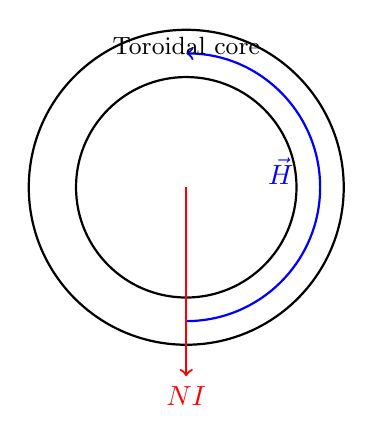
\begin{tikzpicture}
  \draw[thick] (0,0) circle(2);
  \draw[thick] (0,0) circle(1.4);
  \draw[->, thick, blue] (0,-1.7) arc(-90:90:1.7);
  \node[blue] at (1.2,0.2) {\( \vec{H} \)};
  \draw[->, red, thick] (0,0) -- (0,-2.4) node[below] {\( N I \)};
  \node at (0,1.8) {\small Toroidal core};
\end{tikzpicture}
\end{center}



\section*{Example 6-18: Magnetic Energy Stored in an Inductor}

\textbf{Problem:}  
An inductor with inductance \( L \) carries current \( I \). Find the magnetic energy stored and represent the circuit element.

\textbf{Solution:}

Magnetic energy stored is given by:
\[
W = \frac{1}{2} L I^2
\]

\begin{tcolorbox}
\[
\boxed{W = \frac{1}{2} L I^2}
\]
\end{tcolorbox}

\textbf{Diagram:}
\begin{center}
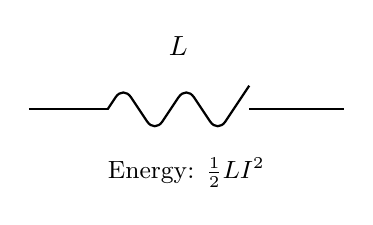
\begin{tikzpicture}
  \draw[thick] (0,0) -- (1,0);
  \draw[thick, rounded corners=5pt] (1,0) -- (1.2,0.3) -- (1.6,-0.3) -- (2,0.3) -- (2.4,-0.3) -- (2.8,0.3);
  \draw[thick] (2.8,0) -- (4,0);
  \node at (1.9,0.8) {\( L \)};
  \node at (2,-0.8) {\small Energy: \( \frac{1}{2} L I^2 \)};
\end{tikzpicture}
\end{center}



\section*{Example 6-19: Force on a Current Loop in a Magnetic Field}

\textbf{Problem:}  
A rectangular loop of current \( I \) lies in a uniform magnetic field \( \vec{B} \). Find the net force on the loop.

\textbf{Solution:}

The magnetic force on each segment:
\[
\vec{F} = I \vec{l} \times \vec{B}
\]

For opposite segments, forces cancel due to symmetry. So:
- Net force is zero in uniform field
- Torque may exist depending on orientation

\begin{tcolorbox}
\[
\boxed{\vec{F}_{\text{net}} = 0 \text{ (in uniform } \vec{B} \text{)}}
\]
\end{tcolorbox}

\textbf{Diagram:}
\begin{center}
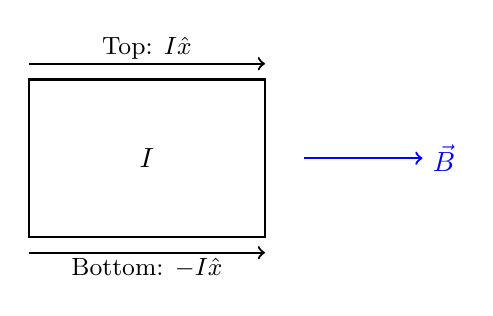
\begin{tikzpicture}
  \draw[thick] (0,0) rectangle (3,2);
  \draw[->, thick, blue] (3.5,1) -- (5,1) node[right] {\( \vec{B} \)};
  \node at (1.5,1) {\( I \)};
  \draw[->, thick] (0,2.2) -- (3,2.2);
  \node at (1.5,2.4) {\small Top: \( I \hat{x} \)};
  \draw[->, thick] (0,-0.2) -- (3,-0.2);
  \node at (1.5,-0.4) {\small Bottom: \( -I \hat{x} \)};
\end{tikzpicture}
\end{center}



\section*{Example 6-20: Torque on a Current Loop in a Magnetic Field}

\textbf{Problem:}  
A rectangular loop of area \( A \), carrying current \( I \), lies in a uniform magnetic field \( \vec{B} \). Find the torque acting on it.

\textbf{Solution:}

The magnetic dipole moment:
\[
\vec{m} = I \vec{A}
\]

Torque on the loop:
\[
\vec{\tau} = \vec{m} \times \vec{B}
\]

If loop is tilted at angle \( \theta \), magnitude of torque:
\[
\tau = I A B \sin\theta
\]

\begin{tcolorbox}
\[
\boxed{\vec{\tau} = \vec{m} \times \vec{B}}, \quad
\boxed{\tau = I A B \sin\theta}
\]
\end{tcolorbox}

\textbf{Diagram:}
\begin{center}
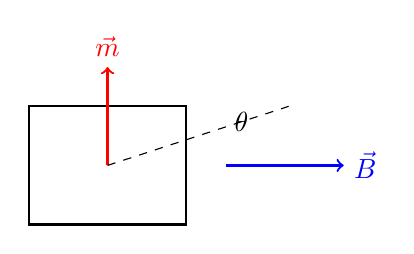
\begin{tikzpicture}
  \draw[thick] (0,0) -- (2,0) -- (2,1.5) -- (0,1.5) -- cycle;
  \draw[->, thick, blue] (2.5,0.75) -- (4,0.75) node[right] {\( \vec{B} \)};
  \draw[->, thick, red] (1,0.75) -- (1,2) node[above] {\( \vec{m} \)};
  \draw[dashed] (1,0.75) -- (3.3,1.5);
  \node at (2.7,1.3) {\( \theta \)};
\end{tikzpicture}
\end{center}



\section*{Example 6-21: Magnetic Boundary Conditions}

\textbf{Problem:}  
Two magnetic materials meet at a boundary with surface current density \( \vec{K}_s \). Determine the boundary conditions for \( \vec{B} \) and \( \vec{H} \).

\textbf{Solution:}

\textbf{Boundary Conditions:}
\[
\hat{n} \cdot (\vec{B}_2 - \vec{B}_1) = 0
\quad \text{(normal component of } \vec{B} \text{ continuous)}
\]
\[
\hat{n} \times (\vec{H}_2 - \vec{H}_1) = \vec{K}_s
\quad \text{(tangential component of } \vec{H} \text{ discontinuous)}
\]

\begin{tcolorbox}
\[
\boxed{
\begin{aligned}
\hat{n} \cdot (\vec{B}_2 - \vec{B}_1) &= 0 \\
\hat{n} \times (\vec{H}_2 - \vec{H}_1) &= \vec{K}_s
\end{aligned}
}
\]
\end{tcolorbox}

\textbf{Diagram:}
\begin{center}
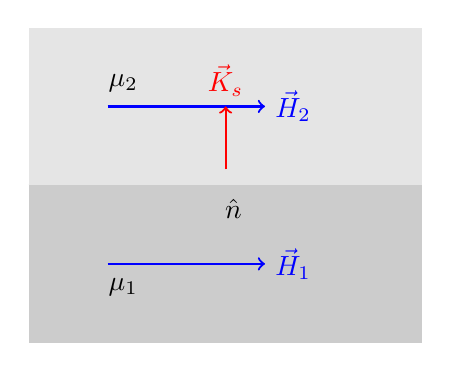
\begin{tikzpicture}
  \draw[thick] (0,0) -- (5,0);
  \fill[gray!20] (0,0) rectangle (5,2);
  \fill[gray!40] (0,0) rectangle (5,-2);
  \node at (1.2,1.3) {\( \mu_2 \)};
  \node at (1.2,-1.3) {\( \mu_1 \)};
  \draw[->, thick, blue] (1,1) -- (3,1) node[right] {\( \vec{H}_2 \)};
  \draw[->, thick, blue] (1,-1) -- (3,-1) node[right] {\( \vec{H}_1 \)};
  \draw[->, thick, red] (2.5,0.2) -- (2.5,1) node[above] {\( \vec{K}_s \)};
  \node at (2.6,-0.3) {\( \hat{n} \)};
\end{tikzpicture}
\end{center}



\section*{Example 6-22: Bound Currents in a Uniformly Magnetized Cylinder}

\textbf{Problem:}  
A long cylinder is uniformly magnetized along its axis with magnetization \( \vec{M} = M_0 \hat{z} \). Find the bound surface and volume currents.

\textbf{Solution:}

The bound volume current is:
\[
\vec{J}_b = \nabla \times \vec{M} = 0 \quad \text{(since } \vec{M} \text{ is constant)}
\]

The bound surface current is:
\[
\vec{K}_b = \vec{M} \times \hat{n} = M_0 \hat{z} \times \hat{r} = M_0 \hat{\phi}
\]

\begin{tcolorbox}
\[
\boxed{\vec{J}_b = 0}, \quad \boxed{\vec{K}_b = M_0 \hat{\phi}}
\]
\end{tcolorbox}

\textbf{Diagram:}
\begin{center}
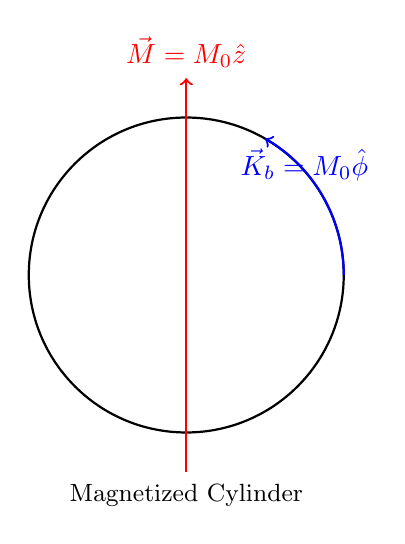
\begin{tikzpicture}
  \draw[thick] (0,0) circle(2);
  \draw[->, thick, red] (0,-2.5) -- (0,2.5) node[above] {\( \vec{M} = M_0 \hat{z} \)};
  \draw[->, thick, blue] (2,0) arc(0:60:2);
  \node[blue] at (1.5,1.4) {\( \vec{K}_b = M_0 \hat{\phi} \)};
  \node at (0,-2.8) {\small Magnetized Cylinder};
\end{tikzpicture}
\end{center}



\section*{Example 6-23: Magnetic Energy Stored in Terms of \( \vec{H} \)}

\textbf{Problem:}  
Express the total magnetic energy stored in a volume in terms of the magnetic field \( \vec{H} \) and permeability \( \mu \).

\textbf{Solution:}

Magnetic energy density is:
\[
u = \frac{1}{2} \mu H^2
\]

Total energy:
\[
W = \int_V u \, dV = \int_V \frac{1}{2} \mu H^2 \, dV
\]

\begin{tcolorbox}
\[
\boxed{W = \int_V \frac{1}{2} \mu H^2 \, dV}
\]
\end{tcolorbox}

\textbf{Diagram:}
\begin{center}
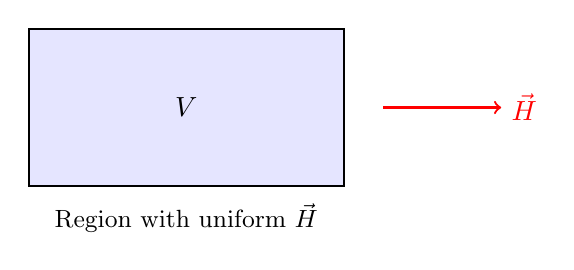
\begin{tikzpicture}
  \draw[fill=blue!10, thick] (0,0) rectangle (4,2);
  \node at (2,1) {\( V \)};
  \draw[->, thick, red] (4.5,1) -- (6,1) node[right] {\( \vec{H} \)};
  \node at (2,-0.4) {\small Region with uniform \( \vec{H} \)};
\end{tikzpicture}
\end{center}



\section*{Example 6-24: Magnetic Force as Gradient of Energy}

\textbf{Problem:}  
Show how the magnetic force on a system can be expressed as the gradient of magnetic energy.

\textbf{Solution:}

Magnetic energy stored in an inductor:
\[
W = \frac{1}{2} L I^2
\]

If inductance \( L \) depends on position \( x \), then:
\[
F = -\frac{dW}{dx} = -\frac{1}{2} I^2 \frac{dL}{dx}
\]

This force is directed toward increasing inductance (e.g., closing magnetic gaps).

\begin{tcolorbox}
\[
\boxed{F = -\frac{d}{dx} \left( \frac{1}{2} L I^2 \right) = -\frac{1}{2} I^2 \frac{dL}{dx}}
\]
\end{tcolorbox}

\textbf{Diagram:}
\begin{center}
\begin{tikzpicture}
  \draw[thick] (0,0) rectangle (1,2);
  \draw[thick] (3,0) rectangle (4,2);
  \draw[fill=gray!20] (1,0.8) rectangle (3,1.2);
  \draw[->, thick, red] (2,2.2) -- (2,3) node[above] {\( \vec{F} \)};
  \node at (2,0.4) {\small Magnetic gap};
  \node at (2,-0.5) {\small Variable gap ⇒ \( L(x) \)};
\end{tikzpicture}
\end{center}



\section*{Problem P.6-41: Magnetic Field from Current Sheet Pair}

\textbf{Problem:}  
Two infinite, parallel current sheets lie in the \( xy \)-plane at \( z = \pm d \). Each carries a surface current \( K \hat{x} \), in opposite directions. Find the magnetic field \( \vec{B} \) in all regions.

\textbf{Solution:}

Use Ampère’s Law in three regions:

- Above the top sheet (\( z > d \)):  
  Fields from both sheets cancel ⇒ \( \vec{B} = 0 \)

- Between the sheets (\( -d < z < d \)):  
  \[
  \vec{B} = \mu_0 K \hat{y}
  \]

- Below the bottom sheet (\( z < -d \)):  
  Fields cancel ⇒ \( \vec{B} = 0 \)

\begin{tcolorbox}
\[
\boxed{
\vec{B}(z) =
\begin{cases}
0, & z > d \\
\mu_0 K \hat{y}, & -d < z < d \\
0, & z < -d
\end{cases}
}
\]
\end{tcolorbox}

\textbf{Diagram:}
\begin{center}
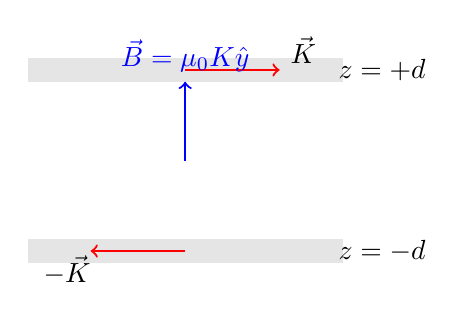
\begin{tikzpicture}
  \fill[gray!20] (-2,1) rectangle (2,1.3);
  \fill[gray!20] (-2,-1.3) rectangle (2,-1);
  \node at (2.5,1.15) {\( z = +d \)};
  \node at (2.5,-1.15) {\( z = -d \)};
  \draw[->, thick, red] (0,1.15) -- (1.2,1.15);
  \draw[->, thick, red] (0,-1.15) -- (-1.2,-1.15);
  \node at (1.5,1.4) {\( \vec{K} \)};
  \node at (-1.5,-1.4) {\( -\vec{K} \)};
  \draw[->, thick, blue] (0,0) -- (0,1) node[above] {\( \vec{B} = \mu_0 K \hat{y} \)};
\end{tikzpicture}
\end{center}



\section*{Problem P.6-42: Magnetic Energy in a Cylindrical Shell}

\textbf{Problem:}  
A long cylindrical shell of inner radius \( a \) and outer radius \( b \) carries a uniform current density \( J \hat{z} \). Compute the total magnetic energy stored per unit length.

\textbf{Solution:}

1. Compute magnetic field in the shell \( (a < r < b) \):

\[
I_{\text{enc}}(r) = J \pi (r^2 - a^2)
\]
\[
B(r) = \frac{\mu_0 I_{\text{enc}}}{2\pi r} = \frac{\mu_0 J (r^2 - a^2)}{2r}
\]

2. Magnetic energy density:
\[
u = \frac{B^2}{2\mu_0}
\]

3. Total energy per unit length:
\[
W = \int_a^b \frac{1}{2\mu_0} \left( \frac{\mu_0 J (r^2 - a^2)}{2r} \right)^2 2\pi r \, dr
= \frac{\mu_0 \pi J^2}{2} \int_a^b \frac{(r^2 - a^2)^2}{r} \, dr
\]

Leave result in integral form unless numeric evaluation is required.

\begin{tcolorbox}
\[
\boxed{W = \frac{\mu_0 \pi J^2}{2} \int_a^b \frac{(r^2 - a^2)^2}{r} \, dr}
\]
\end{tcolorbox}

\textbf{Diagram:}
\begin{center}
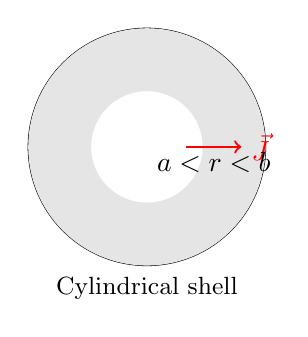
\begin{tikzpicture}
  \draw[thick] (0,0) circle(1.5);
  \draw[thick] (0,0) circle(0.7);
  \filldraw[gray!20] (0,0) circle(1.5);
  \filldraw[white] (0,0) circle(0.7);
  \draw[->, thick, red] (0.5,0) -- (1.2,0) node[right] {\( \vec{J} \)};
  \node at (0.85,-0.2) {\( a < r < b \)};
  \node at (0,-1.8) {\small Cylindrical shell};
\end{tikzpicture}
\end{center}



\section*{Problem P.6-43: Magnetic Force Between Two Parallel Wires}

\textbf{Problem:}  
Two long parallel wires separated by distance \( d \) carry currents \( I_1 \) and \( I_2 \) in the same direction. Find the force per unit length on one wire due to the other.

\textbf{Solution:}

Magnetic field from wire 1 at location of wire 2:
\[
B_1 = \frac{\mu_0 I_1}{2\pi d}
\]

Force on wire 2:
\[
F_{21} = I_2 L \times B_1 \Rightarrow \frac{F_{21}}{L} = I_2 B_1 = \frac{\mu_0 I_1 I_2}{2\pi d}
\]

Direction: Attractive if currents are in same direction, repulsive if opposite.

\begin{tcolorbox}
\[
\boxed{\frac{F}{L} = \frac{\mu_0 I_1 I_2}{2\pi d}}
\]
\end{tcolorbox}

\textbf{Diagram:}
\begin{center}
\begin{tikzpicture}
  \draw[thick] (0,-1.5) -- (0,1.5);
  \draw[thick] (3,-1.5) -- (3,1.5);
  \node at (-0.3,1.3) {\( I_1 \)};
  \node at (3.3,1.3) {\( I_2 \)};
  \draw[->, thick, red] (0,0) -- (3,0);
  \node at (1.5,0.3) {\( d \)};
  \draw[->, thick, blue] (3,0) -- (3.5,0.5) node[right] {\( \vec{F}_{21} \)};
  \node at (1.5,-1.2) {\small Same direction ⇒ Attraction};
\end{tikzpicture}
\end{center}



\section*{Problem P.6-44: Field on Axis of Finite-Length Current Segment}

\textbf{Problem:}  
A straight wire segment of length \( 2L \) lies along the \( z \)-axis, centered at the origin, carrying current \( I \). Find the magnetic field \( \vec{B} \) at point \( P \) on the \( x \)-axis at distance \( x \).

\textbf{Solution:}

Using Biot–Savart Law for a finite segment:
\[
\vec{B} = \frac{\mu_0 I}{4\pi x} \left( \frac{z_2}{\sqrt{x^2 + z_2^2}} - \frac{z_1}{\sqrt{x^2 + z_1^2}} \right) \hat{y}
\]
Here \( z_1 = -L \), \( z_2 = +L \):
\[
\vec{B} = \frac{\mu_0 I}{4\pi x} \left( \frac{L}{\sqrt{x^2 + L^2}} - \frac{-L}{\sqrt{x^2 + L^2}} \right) \hat{y}
= \frac{\mu_0 I L}{2\pi x \sqrt{x^2 + L^2}} \hat{y}
\]

\begin{tcolorbox}
\[
\boxed{\vec{B} = \frac{\mu_0 I L}{2\pi x \sqrt{x^2 + L^2}} \hat{y}}
\]
\end{tcolorbox}

\textbf{Diagram:}
\begin{center}
\begin{tikzpicture}
  \draw[thick] (0,-2) -- (0,2);
  \draw[fill=black] (0,-2) circle(0.05) node[left] {\( -L \)};
  \draw[fill=black] (0,2) circle(0.05) node[left] {\( +L \)};
  \draw[->, thick, red] (0,0) -- (2,0) node[right] {\( x \)};
  \draw[dashed] (2,0) -- (2,2);
  \draw[dashed] (2,0) -- (2,-2);
  \node at (2.3,1.5) {\( \sqrt{x^2 + L^2} \)};
  \node at (1,-0.3) {\( P \)};
  \node at (0.3,1) {\( I \)};
\end{tikzpicture}
\end{center}



\section*{Problem P.6-45: Inductance of Two Concentric Cylindrical Shells}

\textbf{Problem:}  
Two infinitely long, thin-walled concentric cylindrical conductors of radii \( a \) and \( b \) (\( b > a \)) carry equal and opposite currents \( I \). Determine the inductance per unit length between them.

\textbf{Solution:}

The magnetic field exists only in the region \( a < r < b \), where:
\[
B(r) = \frac{\mu_0 I}{2\pi r}
\]

Magnetic energy per unit length:
\[
W = \int_a^b \frac{1}{2\mu_0} B^2 \cdot 2\pi r \, dr
= \int_a^b \frac{1}{2\mu_0} \left( \frac{\mu_0 I}{2\pi r} \right)^2 \cdot 2\pi r \, dr
= \frac{\mu_0 I^2}{4\pi} \int_a^b \frac{1}{r} \, dr
\]

\[
W = \frac{\mu_0 I^2}{4\pi} \ln\left( \frac{b}{a} \right)
\]

Since \( W = \frac{1}{2} L I^2 \), we solve for \( L \):
\[
L = \frac{\mu_0}{2\pi} \ln\left( \frac{b}{a} \right)
\]

\begin{tcolorbox}
\[
\boxed{L = \frac{\mu_0}{2\pi} \ln\left( \frac{b}{a} \right)} \quad \text{(per unit length)}
\]
\end{tcolorbox}

\textbf{Diagram:}
\begin{center}
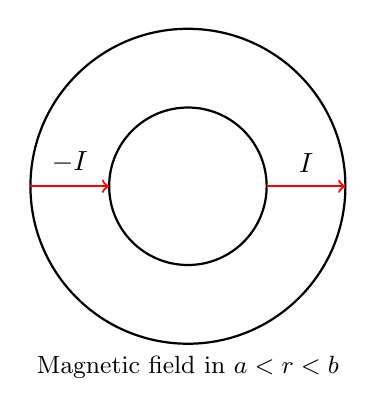
\begin{tikzpicture}
  \draw[thick] (0,0) circle(1);
  \draw[thick] (0,0) circle(2);
  \draw[->, thick, red] (1,0) -- (2,0);
  \draw[->, thick, red] (-2,0) -- (-1,0);
  \node at (1.5,0.3) {\( I \)};
  \node at (-1.5,0.3) {\( -I \)};
  \node at (0,-2.3) {\small Magnetic field in \( a < r < b \)};
\end{tikzpicture}
\end{center}



\section*{Problem P.6-46: Inductance of Parallel Wire Transmission Line}

\textbf{Problem:}  
Two parallel wires of radius \( a \), spaced a distance \( d \gg a \) apart, carry equal and opposite currents \( I \). Derive the inductance per unit length.

\textbf{Solution:}

The magnetic field between the wires is approximated using superposition:
\[
B = \frac{\mu_0 I}{2\pi r}, \quad a < r < d-a
\]

Energy per unit length:
\[
W = \int_a^{d-a} \frac{1}{2\mu_0} B^2 \cdot 2\pi r \, dr
= \int_a^{d-a} \frac{1}{2\mu_0} \left( \frac{\mu_0 I}{2\pi r} \right)^2 \cdot 2\pi r \, dr
= \frac{\mu_0 I^2}{4\pi} \int_a^{d-a} \frac{1}{r} \, dr
\]

\[
W = \frac{\mu_0 I^2}{4\pi} \ln\left( \frac{d-a}{a} \right)
\Rightarrow L = \frac{\mu_0}{2\pi} \ln\left( \frac{d-a}{a} \right)
\]

If \( d \gg a \), then \( d-a \approx d \):
\[
\boxed{L = \frac{\mu_0}{2\pi} \ln\left( \frac{d}{a} \right)}
\]

\begin{tcolorbox}
\[
\boxed{L = \frac{\mu_0}{2\pi} \ln\left( \frac{d}{a} \right)} \quad \text{(per unit length)}
\]
\end{tcolorbox}

\textbf{Diagram:}
\begin{center}
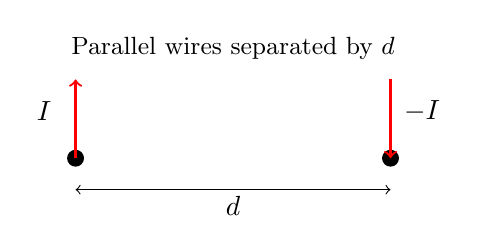
\begin{tikzpicture}
  \draw[fill=black] (-2,0) circle(0.1);
  \draw[fill=black] (2,0) circle(0.1);
  \draw[->, thick, red] (-2,0) -- (-2,1);
  \draw[->, thick, red] (2,1) -- (2,0);
  \node at (-2.4,0.6) {\( I \)};
  \node at (2.4,0.6) {\( -I \)};
  \draw[<->] (-2, -0.4) -- (2, -0.4);
  \node at (0, -0.6) {\( d \)};
  \node at (0, 1.4) {\small Parallel wires separated by \( d \)};
\end{tikzpicture}
\end{center}



\section*{Problem P.6-47: Self-Inductance of a Square Loop}

\textbf{Problem:}  
Find the self-inductance of a square loop of side length \( l \) carrying current \( I \), assuming the wire has small radius \( a \) and \( l \gg a \).

\textbf{Solution:}

The magnetic flux through the loop due to its own current is estimated using Neumann’s formula or known result for a loop:

\[
L \approx \mu_0 l \left[ \ln\left( \frac{2l}{a} \right) - 0.774 \right]
\]

This is a standard approximation valid for thin wires forming a square.

\begin{tcolorbox}
\[
\boxed{L \approx \mu_0 l \left[ \ln\left( \frac{2l}{a} \right) - 0.774 \right]}
\]
\end{tcolorbox}

\textbf{Diagram:}
\begin{center}
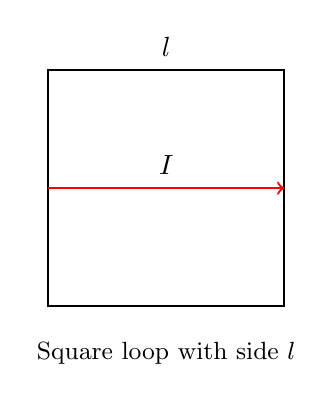
\begin{tikzpicture}
  \draw[thick] (0,0) rectangle (3,3);
  \node at (1.5,3.3) {\( l \)};
  \draw[->, thick, red] (0,1.5) -- (3,1.5);
  \node at (1.5,1.8) {\( I \)};
  \node at (1.5,-0.6) {\small Square loop with side \( l \)};
\end{tikzpicture}
\end{center}



\section*{Problem P.6-48: Mutual Inductance Between Two Coaxial Loops}

\textbf{Problem:}  
Two circular loops of radii \( R_1 \) and \( R_2 \) are placed coaxially and separated by distance \( d \). Find the mutual inductance \( M \) between them assuming \( R_1, R_2 \ll d \).

\textbf{Solution:}

Approximate the magnetic field at the second loop due to the first using dipole approximation:
\[
B = \frac{\mu_0 I \pi R_1^2}{2\pi d^3}
\]

Flux through second loop:
\[
\Phi = B \cdot \pi R_2^2 = \frac{\mu_0 I \pi R_1^2 \cdot \pi R_2^2}{2\pi d^3}
= \frac{\mu_0 \pi^2 R_1^2 R_2^2}{2 d^3} I
\]

Mutual inductance:
\[
M = \frac{\Phi}{I} = \frac{\mu_0 \pi^2 R_1^2 R_2^2}{2 d^3}
\]

\begin{tcolorbox}
\[
\boxed{M = \frac{\mu_0 \pi^2 R_1^2 R_2^2}{2 d^3}}
\]
\end{tcolorbox}

\textbf{Diagram:}
\begin{center}
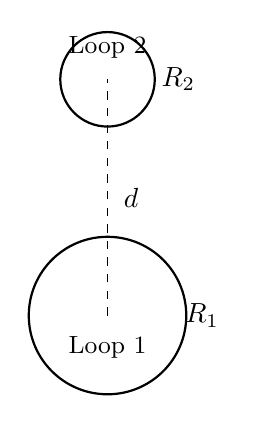
\begin{tikzpicture}
  \draw[thick] (0,0) circle(1);
  \draw[thick] (0,3) circle(0.6);
  \draw[dashed] (0,0) -- (0,3);
  \node at (0.3,1.5) {\( d \)};
  \node at (1.2,0) {\( R_1 \)};
  \node at (0.9,3) {\( R_2 \)};
  \node at (0,-0.4) {\small Loop 1};
  \node at (0,3.4) {\small Loop 2};
\end{tikzpicture}
\end{center}



\section*{Problem P.6-49: Field Inside a Toroid with Square Cross Section}

\textbf{Problem:}  
A toroidal coil has \( N \) turns and carries current \( I \). The core has a square cross section of side \( a \) and mean radius \( R \). Find the magnetic field \( \vec{B} \) inside the toroid.

\textbf{Solution:}

Using Ampère’s Law around a circular path inside the core:
\[
\oint \vec{B} \cdot d\vec{l} = B \cdot 2\pi r = \mu_0 N I
\Rightarrow B(r) = \frac{\mu_0 N I}{2\pi r}, \quad R - \frac{a}{2} < r < R + \frac{a}{2}
\]

\begin{tcolorbox}
\[
\boxed{B(r) = \frac{\mu_0 N I}{2\pi r}} \quad \text{(inside the core)}
\]
\end{tcolorbox}

\textbf{Diagram:}
\begin{center}
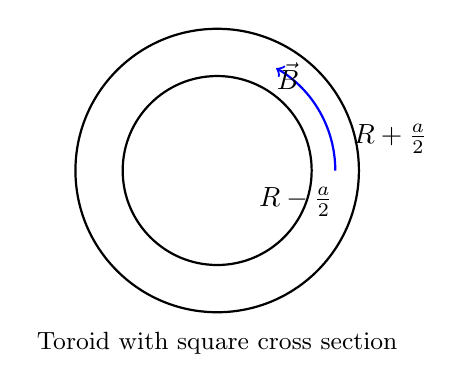
\begin{tikzpicture}
  \draw[thick] (0,0) circle(1.8);
  \draw[thick] (0,0) circle(1.2);
  \node at (2.2,0.4) {\( R + \frac{a}{2} \)};
  \node at (1.0,-0.4) {\( R - \frac{a}{2} \)};
  \draw[->, thick, blue] (0,0) ++(1.5,0) arc(0:60:1.5);
  \node at (0.9,1.2) {\( \vec{B} \)};
  \node at (0,-2.2) {\small Toroid with square cross section};
\end{tikzpicture}
\end{center}



\section*{Problem P.6-50: Magnetic Energy Stored in a Toroid}

\textbf{Problem:}  
A toroid with \( N \) turns, current \( I \), mean radius \( R \), and cross-sectional area \( A \) is made of a linear magnetic material with permeability \( \mu \). Compute the magnetic energy stored in the core.

\textbf{Solution:}

Magnetic field in toroid:
\[
B = \frac{\mu N I}{2\pi R}
\]

Energy density:
\[
u = \frac{B^2}{2\mu}
\]

Volume of core: \( V = 2\pi R \cdot A \)

Total energy:
\[
W = u \cdot V = \frac{1}{2\mu} \left( \frac{\mu N I}{2\pi R} \right)^2 \cdot 2\pi R A
= \frac{\mu N^2 I^2 A}{4\pi R}
\]

\begin{tcolorbox}
\[
\boxed{W = \frac{\mu N^2 I^2 A}{4\pi R}}
\]
\end{tcolorbox}

\textbf{Diagram:}
\begin{center}
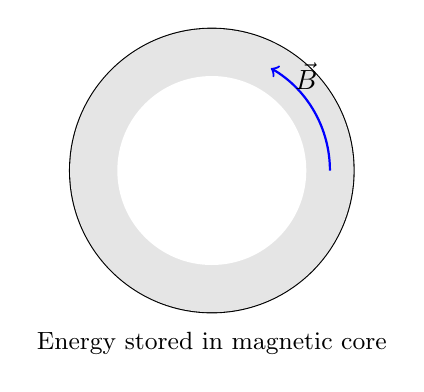
\begin{tikzpicture}
  \draw[thick] (0,0) circle(1.8);
  \draw[thick] (0,0) circle(1.2);
  \fill[gray!20] (0,0) circle(1.8);
  \fill[white] (0,0) circle(1.2);
  \draw[->, thick, blue] (1.5,0) arc(0:60:1.5);
  \node at (1.2,1.2) {\( \vec{B} \)};
  \node at (0,-2.2) {\small Energy stored in magnetic core};
\end{tikzpicture}
\end{center}



\section*{Problem P.6-51: Force Between Two Parallel Current Sheets}

\textbf{Problem:}  
Two infinite parallel current sheets, each carrying surface current density \( \vec{K} = K \hat{x} \), are located at \( z = \pm d \), with currents in the same direction. Find the force per unit area between the sheets.

\textbf{Solution:}

Magnetic field between the sheets:
\[
\vec{B} = \mu_0 K \hat{y}
\]

Force per unit length on one sheet:
\[
\vec{F} = \vec{K} \times \vec{B} = K \hat{x} \times \mu_0 K \hat{y} = \mu_0 K^2 \hat{z}
\]

So, the force per unit area is:
\[
\frac{F}{A} = \mu_0 K^2
\]

Direction: Repulsive (since \( \vec{K} \times \vec{B} \) points away from the other sheet)

\begin{tcolorbox}
\[
\boxed{\frac{F}{A} = \mu_0 K^2}
\]
\end{tcolorbox}

\textbf{Diagram:}
\begin{center}
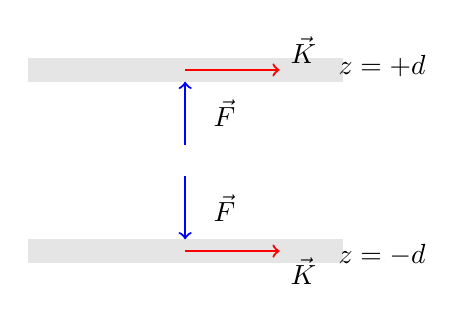
\begin{tikzpicture}
  \fill[gray!20] (-2,1) rectangle (2,1.3);
  \fill[gray!20] (-2,-1.3) rectangle (2,-1);
  \draw[->, thick, red] (0,1.15) -- (1.2,1.15);
  \draw[->, thick, red] (0,-1.15) -- (1.2,-1.15);
  \node at (1.5,1.4) {\( \vec{K} \)};
  \node at (1.5,-1.4) {\( \vec{K} \)};
  \draw[->, thick, blue] (0,0.2) -- (0,1);
  \draw[->, thick, blue] (0,-0.2) -- (0,-1);
  \node at (0.5,0.6) {\( \vec{F} \)};
  \node at (0.5,-0.6) {\( \vec{F} \)};
  \node at (2.5,1.2) {\( z = +d \)};
  \node at (2.5,-1.2) {\( z = -d \)};
\end{tikzpicture}
\end{center}



\section*{Problem P.6-52: Magnetic Vector Potential of an Infinite Line Current}

\textbf{Problem:}  
An infinite straight wire along the \( z \)-axis carries current \( I \). Determine the magnetic vector potential \( \vec{A} \) in cylindrical coordinates.

\textbf{Solution:}

We use the known symmetry and relationship:
\[
\vec{B} = \nabla \times \vec{A}
\]

From Ampère’s Law:
\[
\vec{B} = \frac{\mu_0 I}{2\pi r} \hat{\phi}
\]

We choose:
\[
\vec{A} = A_z(r) \hat{z}
\]

Then:
\[
\nabla \times \vec{A} = \left( \frac{1}{r} \frac{d}{dr}(r A_z) \right) \hat{\phi} = \vec{B}
\Rightarrow \frac{1}{r} \frac{d}{dr}(r A_z) = \frac{\mu_0 I}{2\pi r}
\]

Multiply both sides by \( r \) and integrate:
\[
\frac{d}{dr}(r A_z) = \frac{\mu_0 I}{2\pi} \Rightarrow r A_z = \frac{\mu_0 I}{2\pi} r + C
\Rightarrow A_z = \frac{\mu_0 I}{2\pi} \ln r + \frac{C}{r}
\]

Neglecting \( \frac{C}{r} \) for large \( r \), we take:
\[
\vec{A} = \frac{\mu_0 I}{2\pi} \ln r \, \hat{z}
\]

\begin{tcolorbox}
\[
\boxed{\vec{A}(r) = \frac{\mu_0 I}{2\pi} \ln r \, \hat{z}}
\]
\end{tcolorbox}

\textbf{Diagram:}
\begin{center}
\begin{tikzpicture}
  \draw[thick] (0,-2) -- (0,2);
  \draw[->, thick, red] (0,0) -- (1.5,0);
  \node at (1.8,0) {\( r \)};
  \node at (0.4,1) {\( I \)};
  \node at (1,-0.4) {\( \vec{A} \parallel \hat{z} \)};
\end{tikzpicture}
\end{center}



\section*{Problem P.6-53: Magnetic Field from a Given Vector Potential}

\textbf{Problem:}  
A magnetic vector potential is given as \( \vec{A}(x, y, z) = A_0 x \hat{z} \). Determine the corresponding magnetic field \( \vec{B} \).

\textbf{Solution:}

We use the relation:
\[
\vec{B} = \nabla \times \vec{A}
\]

Given:
\[
\vec{A} = A_0 x \hat{z}
\]

Compute the curl:
\[
\nabla \times \vec{A} =
\begin{vmatrix}
\hat{x} & \hat{y} & \hat{z} \\
\partial_x & \partial_y & \partial_z \\
0 & 0 & A_0 x
\end{vmatrix}
= \left( 0 - 0 \right)\hat{x} - \left( 0 - 0 \right)\hat{y} + \left( 0 - 0 \right)\hat{z} + A_0 \hat{y}
= -A_0 \hat{y}
\]

\begin{tcolorbox}
\[
\boxed{\vec{B} = -A_0 \hat{y}}
\]
\end{tcolorbox}

\textbf{Diagram:}
\begin{center}
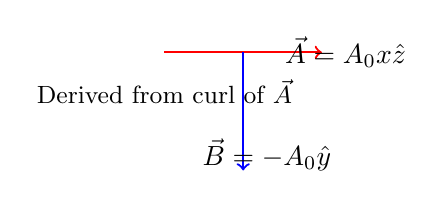
\begin{tikzpicture}
  \draw[->, thick, red] (0,0) -- (2,0);
  \node at (2.3,0) {\( \vec{A} = A_0 x \hat{z} \)};
  \draw[->, thick, blue] (1,0) -- (1,-1.5);
  \node at (1.3,-1.3) {\( \vec{B} = -A_0 \hat{y} \)};
  \node at (0,-0.5) {\small Derived from curl of \( \vec{A} \)};
\end{tikzpicture}
\end{center}


\end{document}